\chapter{L'environnement Hardware}\label{chap:environement-materiel-requis}
\index{environnement hardware}

\chapintro{Ce chapitre discute des composantes mat\'erielles
n\'ecessaires pour le bon fonctionnement de \yeren.}

\nxsection{La m\'emoire RAM}
\index{m\'emoire RAM}
\index{m\'emoire vive}

\yeren peut \^etre utilis\'e sur un ordinateur qui
poss\`ede un minimum de $512$ Mo de m\'emoire RAM
(m\'emoire vive) sans aucun probl\`eme.

Cependant, nous recommendons l'utilisation d'ordinateurs
ayant un minimum de $2$ Go de m\'emoire RAM.

%-------------------------------------------------------------

\nxsection{Le disque dur}
\index{disque dur}

L'utilisateur de \yeren doit se pr\'emunir d'un disque
dur en fonction de la quantit\'e de donn\'ees qu'il
pr\'evoit stocker dans la base de donn\'ees.

\yeren n'a pas de requis quant \`a la capacit\'e
des disques durs du client. C'est le syst\`eme d'exploitation
et le syst\`eme de gestion de base de donn\'ees (SGBD)
utilis\'e qui conditionnent la capacit\'e des disques
durs \`a utiliser.

%-------------------------------------------------------------

\newpage

\nxsection{Le Mat\'eriel Informatique Recommand\'e}
\index{mat\'eriel informatique recommand\'e}

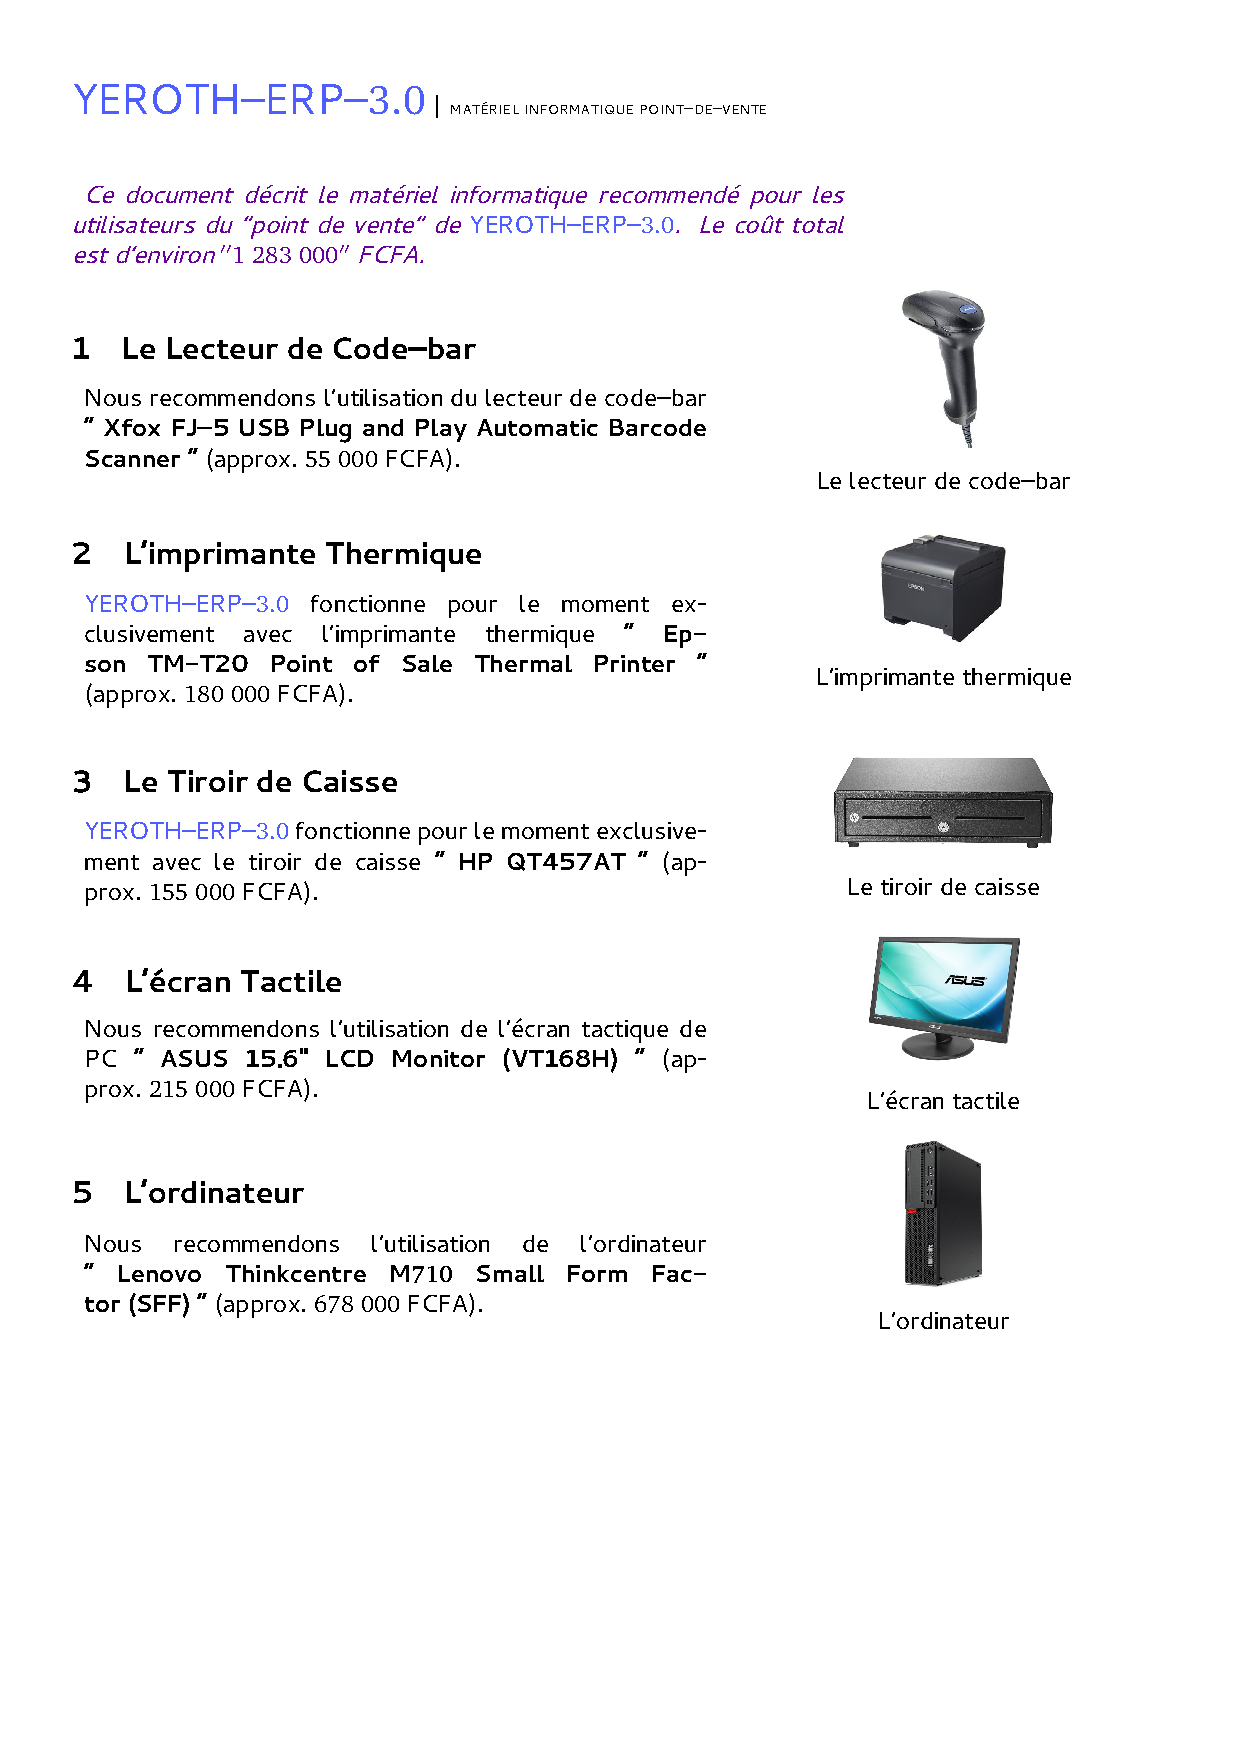
\includegraphics[scale=0.86]{../yeroth-white-papers/yeroth-erp-3-0-PDV-materiel-informatique-recommende.pdf}
